%%% Template File for Use with the hmcthesis.cls.
%%%
%%% C.M. Connelly <cmc@math.hmc.edu>
%%%
%%% Version 5.1


%%% !!! HMC STUDENTS SHOULD REMOVE THE FOLLOWING COPYRIGHT NOTICE FROM
%%% !!! FINAL SUBMISSIONS.

%%% Copyright (C) 2004-2015 Department of Mathematics, Harvey Mudd College.
%%%
%%% This file is part of the sample thesis provided to HMC
%%% mathematics students and is based on the sample thesis's
%%% master.tex file.  Please see that file for more information.

%%% See the COPYING document, which should accompany this
%%% distribution, for information about distribution and modification
%%% of the document and its components.

%%% !!! END COPYRIGHT NOTICE.

%%% Preamble.

%%% The top part of your document is called the preamble.  You supply
%%% some basic information about the document (such as its title and
%%% author) in a form that LaTeX can understand here.

%%% You can also load additional LaTeX packages, or style files, that
%%% affect the way that the document is laid out, typeset, or supply
%%% additional commands or environments.


%%% Theses use the hmcthesis document class, which should be
%%% located somewhere in TeX's search path.
\documentclass[mathematics]{hmcthesis}

%%% You must set a document-class option to tell the class what
%%% department your report will be for!  Replace the string
%%% <<document>> with the name of a department, where supported
%%% departments are
%%%
%%%    biology
%%%    computer-science
%%%    chemistry
%%%    engineering
%%%    mathematics
%%%    physics


%%% Additional document-class options.

%%% The "sigpage" document-class option generates a signature page
%%% for your thesis, as in

%%% \documentclass[sigpage,<<department>>]{hmcthesis}

%%% The "noamsthm" document-class option stops the amsthm package
%%% from being loaded by the class.  This option is provided in
%%% case you prefer to use some other package to format your
%%% theorems, lemmas, and so on.


%%% Additional packages.

%%% Other packages needed by your document may be loaded here.
%%% with the \usepackage{} command.  If you choose to load
%%% additional packages, make sure that they appear *before* the
%%% line loading hyperref; hyperref changes pieces of other
%%% packages, so it's important that it be loaded last.


%%% The class file loads the following packages -- there is no
%%% reason to load any of these packages yourself (and doing so
%%% may cause problems):
%%%
%%% amsmath, amsfonts, amsthm (unless you specify "noamsmath" in
%%% the document-class options), booktabs, calc, caption, ccicons,
%%% fancyhdr, graphics, ifthen, inconsolata, mathalfa, natbib,
%%% newpxmath, newpxtext, sourcesanspro, textcomp, url, verbatim,
%%% xspace.

% \usepackage{graphicx}           % More control over graphic inclusion.
\usepackage{csquotes}
\usepackage[english]{babel}
\usepackage{pdfpages}
%%% Load all other packages before this point.

%%% Load hyperref.
\usepackage[breaklinks=true,
  bookmarks,
  pdfpagemode=UseOutlines,
  pdfpagelayout=SinglePage]{hyperref}


%%% Your own commands and environments.

%%% The preamble can also be used to define your own commands and
%%% environments, set some constants that will be used throughout your
%%% document, and so on.



%%% As you may have guessed, LaTeX's comment character is the percent
%%% sign.  Any line that starts with a % will be ignored.  You can
%%% also use the comment character to add comments to the end of a
%%% line that will be parsed by TeX.

%%% The optional \includeonly command allows you to specify the names
%%% of chapters that you want to typeset.  It is useful for debugging
%%% or for working intensely on one particular part of your document
%%% when you don't want to take the time to retypeset the entire document.


%%% The first active line in your LaTeX document is the \documentclass
%%% command, which loads a LaTeX class file.  Class files generally
%%% define the appearance of a document, and include a variety of
%%% structural commands.

%%% This optional command provides additional context around an error.
%%% It can be helpful when tracking down a problem.
%\setcounter{errorcontextlines}{1000}


%%% Information about this document.

%%% I find it most useful to put identifying information about a
%%% document near the top of the preamble.  Technically, this
%%% information must precede the \maketitle command, which often
%%% appears immediately after the beginning of the document
%%% environment.  Placing it near the top of the document makes it
%%% easier to identify the document, and keeps it from getting
%%% mixed up with the content of your document.

%%% So, some questions.

%% What is the title of your report?
\title{On Self Regulation in College-Level Mathematics Classes}

%% Who are the authors of the report?  (Separate multiple names with \and.)
\author{Jenny Lee}

%% What is your faculty advisor's name?  (Again, separate names with
%% \and, if necessary.)
%%
%% Don't include titles (e.g., ``Prof.'', ``Dr.'').
\advisor{Dagan Karp}

%% Second reader's name?  If you have a third or fourth reader, add
%%% their names here, separated by the \and command.
%%
%% Don't include titles (e.g., ``Prof.'', ``Dr.'').
\reader{Luis A. Leyva}

%% The year in which you are submitting your thesis.
\thesisyear{2018}

%% Optional: The month in which you are submitting your thesis (if
%% it's a month other than May).  For example,
% \thesismonth{December}

%%% End of information section.


%%% New commands and environments.

%%% You can define your own commands and environments here.  If you
%%% have a lot of material here, you might want to consider splitting
%%% the commands and environments into a separate ``style'' file that
%%% you load with \usepackage.

% \newcommand{\coolcommand}[1]{#1 is cool.} % Lets everyone know that
                                % the person or thing that you provide
                                % as the argument to the command is
                                % cool.

% \newcounter{cms}


%%% Some theorem-like command definitions.

%%% The \newtheorem command comes from the amsthm package.  That
%%% package is *not* loaded by the class file, so if you choose
%%% to use these commands, you'll need to load the package above.

% \newtheorem{thm}{Theorem}[chapter]
% \newtheorem{lem}{Lemma}[chapter]


%%% If you find that some words in your document are being hyphenated
%%% incorrectly, you can specify the correct hyphenation using the
%%% \hyphenation command.  Note that words are separated by
%%% whitespace, as shown below.

\hyphenation{ap-pen-dix wer-ther-i-an}


%%% The start of the document!

%% The document environment is the main environment in any LaTeX
%% document.  It contains other environments, as well as your text.

\begin{document}

%%% The front matter of a large document includes the title page or
%%% pages, tables of contents, lists of figures or tables, and so on,
%%% your abstract, a preface or introduction, and so on.  It's
%%% delineated with the \frontmatter command.

\frontmatter


%%% One of the things that the \frontmatter does is make page
%%% numbers appear as lowercase Roman numerals---i, vi, xii, and so
%%% on.

%%% The first thing in the front matter is your title page.  The title
%%% page is formatted by commands in the document class file, so you
%%% don't need to worry about what it looks like -- just putting the
%%% \maketitle command in your document (and filling in the necessary
%%% information for the identification commands above) is enough.

\maketitle


%%% Abstract

\begin{abstract}
  This paper looks into need for improvement in mathematics education at the college level in the US regarding equitable practices in instruction. In particular, this paper focuses on understanding the role self-regulation can play in the classroom dynamics, and how self-paced assessment can be a way to empower students. Also included is a case study in an introductory linear algebra class at a liberal arts college and is meant to provide a investigation into self-regulation in this context. The appendix includes an annotated bibliography comprised of the most relevant studies in self-regulation conducted in the last two decades or so. An index of keywords and pertinent quotes are highlighted for the ease of the reader.
\end{abstract}


%%% Table of Contents, List of Figures, and List of Tables.
%%%
%%% If you don't have any figures or tables in your report, you
%%% should comment out the appropriate command.  If you don't,
%%% you'll get an extra, mostly blank, page in your typeset report.

\tableofcontents
%%% \listoffigures
%%% \listoftables



%%% Acknowledgments.

\begin{acknowledgments}
%% Thank some people here, if you like.
\end{acknowledgments}

%%% End of the front matter.


%%% Beginning of the main matter.

%% The main part of your report consists of normal, numbered
%% chapters as well as any appendices.  Bibliographies, indexes, and
%% so on are part of the back matter.  The main matter is opened with the
%% \mainmatter command.

\mainmatter


%%% Content.

%%% For smaller documents---especially those you're writing by
%%% yourself---you might write your entire report using a single LaTeX
%%% source file.  For larger documents, we recommend that you split
%%% the source file into several separate, smaller files.  The smaller
%%% files are ``included'' into your main, or ``master'' document
%%% using \include commands.

%%% Splitting your source has several advantages.  First, if you're
%%% working on a document with a group of people, it allows you to
%%% have more than one person working on different parts of the
%%% document at the same time (although we still recommend that you
%%% use CVS or a similar revision-control system!).  Second, smaller
%%% document chunks allow you to reorganize your document more
%%% easily.  If you later decide that Chapter 8 would be better as
%%% Chapter 4, all you have to do is swap the \include commands
%%% around.  For that reason, you should give your separate chapters
%%% meaningful names, such as ``introduction'', ``background'', or
%%% ``conclusions'' rather than calling them ``chapter1'',
%%% ``chapter2'', and so on.
%%%
%%% Finally, splitting the document allows you to concentrate on a
%%% particular section without being distracted by other
%%% sections---all you have to do is comment out the \include line for
%%% the sections you're not working on.  This technique can be
%%% especially useful when you're trying to track down a problem by
%%% allowing you to easily locate the file with the problem by
%%% ruling out the other sections.

%%% In our example document, we define several chapters that have
%%% useful information about writing Clinic or thesis reports or
%%% using LaTeX.  Here, we'll just use placeholders (but not
%%% chapter1, chapter2, etc!).  .


%%% Chapter 1

\chapter{In context, math is not fair.}

\section{The need for change}
I politely ask you to consider: a typical child grows up being told over and over again to ``be quiet'' and to learn the materials presented in front of them; there are no stupid questions as long as they are relevant to the material at hand. As they progress into higher education (if they do), they find themselves often sitting in a large lecture hall, questions left unanswered ``in the interest of time,'' and wondering whether the lecturer knows their name, or even cares if they show up at all.

A Google search for ``changing higher education'' returns a plethora of articles responding to recent student strikes advocating for change in policies regarding finances and other economic concerns. In contrast, a search for ``changing K-12 education'' returns a 20-page ERIC (Education Resources Information Center) document on curriculum reform and effect on entering post-secondary institutions. Despite advances in research in education, classroom instruction has not changed significantly in a typical college in the last five to ten decades, if not more. Students are still attending large lecture-style classes assessed via exams accompanied by weekly, graded assignments. With an increasing number of individuals pursuing a higher education, it seems naive to think that the current systems of education are still suitable or equitable to all students. With the diversifying population of students, it is just as crucial to bring sensible change to promote an equitable learning setting.

\section{Mathematics is not fair}
The current nature of mathematics education in the US provides an extremely different experience for a student who is Asian American versus African American versus white. Starting from achievement gaps between African American and Latino/a students and white students to  the extremely stereotypical belief that ``Asians are good at math,'' there is abundant evidence for the unfair nature of mathematics education \citep{alfinio_flores_examining_2007}.

Specifically, there exists a large socioeconomic difference between ethnicities. The 2007-2011 census provides enough quantitative evidence of the unequal distribution of poverty among different races. American Indians and African Americans came in the highest at about 26\% of the population being in poverty, more than a double in comparison to the 11.6\% of whites \citep{macartney}. A 2018 New York Times article showcasing a megastudy conducted on white and black men showed that of the 5,000 white and 5,000 black boys who grew up in poverty, 48\% of black boys grew up to remain in poverty and only 2\% grew to be rich, while 31\% of white boys remaining in poverty and 10\% became rich (\cite{badger_extensive_2018}).

With income gaps this big, opportunity gaps are not so different. In 2013, enrollment percentages in postsecondary education showed about a near 10\% difference between white (42\%) and black (34\%) students (\cite{musu-gillette_status_nodate}). Graduation rates were similar, lowest for black students at around 41\%. These numbers dip down further for STEM (Science, Technology, Engineering, Mathematics) degrees, about 11\% apart.

Exactly what perpetuates these depressing statistics rests deeply rooted in racism that has lined all of US history. To be more specific, it is absolute ignorance to think that any part of education is void of racism, whether outwardly intentional or not. From the 2005 study conducted by the American Mathematics Society, 80\% of full time mathematics professors with PhDs are white, compared to 1\% black and 2\% Hispanic.

Yet, mathematics is historically not a unique subject to white Europeans; rather, prominent advancements were made by individuals from all over world. Yet, if we ask ourselves the names of famous mathematicians, what we hear are not Srinivasa Ramanujan, Hypatia, or Dorothy Vaughn but rather Euler, Pythagoras and Fermat. The problem in question lies exactly here--whiteness is rarely questioned in this context of mathematics. Without having stood in the shadow of an individual that society pictures to be the ``model mathematician,'' it is extremely difficult to understand the place of inequality in the education of our students. It is the not the white teacher but the student of color who has the sole responsibility to succeed through societal oppression. It is no different than asking an ugly duckling to be something other than what he sees in the reflection.

This lack of having a proper role model impacts the belief a student has that they can succeed, otherwise known as self-efficacy (\cite{thevenin_mentors_2007}). With lowered self-efficacy comes lowered achievement, unsurprisingly (\cite{motlagh_relationship_2011}). Once again, we see how the question of how these unfair societal norms factor into reducing the quality of education or effectiveness of education a student receives is rarely raised.

The solution is not clear either. There are many variables and factors in any classroom environment that either cannot be controlled or are unknown. There is no magic wand that turns poverty-stricken neighborhoods into more privileged ones, nor is there one that removes racial inequality within a school, never-mind school districts across a nation. One important example of an unexpected factor that aggravates the situation is microaggression, which describes any seemingly small behavior, including unvocalized assumptions, that relays hostility or prejudiced views towards a marginalized group, unintentional or not. When unnoticed or ignored, microaggressions towards ethnic minority groups feed racism, fueling a mindset that only continues to be confirmed as a correct one. As a result, impacted students fall further into the mindset of feeling less capable in the classroom.

In particular, this happens in subjects like mathematics, widely believed to be a neutral subject. First, neutrality on its own deserves to be revisited. Statements such as ``all lives matter'' made as a counter to the Black Lives Matter movement, describe a harmful form of using neutrality to deny racism exists. In a similar vein, stating that ``mathematics has no color'' contains as many subliminal messages. As Rochelle Gutierrez, notable for her advocacy in equitable education, writes:
\begin{displayquote}
  {[In]} many mathematics classrooms, students are expected to leave their emotions, their bodies, their cultures, and their values outside the classroom walls, stripping them of a sense of wholeness (\cite{gutierrez_embracing_2012}).
\end{displayquote}
It is not to say that finding a derivative is promoting white supremacy. Rather, the way in which we teach a mathematical concept and the myriad of assumptions we make in the process shape the role mathematics takes in our society. In this light, remodeling education to eliminate inequitable practices in mathematics seems a daunting task for any one nation, let alone an institution, to tackle.

Thus, I propose to look into establishing self-efficacy in students. The status quo continues to marginalize students, undermining their abilities and discouraging them from the simple thought that they can succeed in mathematics. By letting students believe that they are capable and entrusting them with their own capabilities, classrooms will no longer be a place for oppression but a place for opportunity for everyone. Building self-efficacy will hence build supportive environments that can empower students with independence and trust in themselves.

While I believe such an ambition can be achieved in various ways, not excluding political and administrative actions, I think fostering self-regulation is a promising first step. in the next chapter, self-regulation is defined and detailed, showing how it can build an equitable classroom.


%%% Chapter 2

\chapter{Self-Regulation}

\section{Definition}
This is the definition of self-regulation provided by Zeider, Pintrich and Boekaerts' \emph{Handbook of Self-Regulation}:
\begin{displayquote}
  Self-regulation refers to self-generated thoughts, feelings, and actions that are planned and cyclically adapted to the attainment of personal goals (Zeider, et al., 1999).
\end{displayquote}

This can be broken into two parts. First, it focuses on self-generation, indicating the necessity for an individual's own efforts and thus emphasizing power in the self. That way, the generated thoughts and actions can be structured to their own goals and needs, not those of the society or instructor. The word ``cyclically'' should be underlined here, as it points out how the process can be a self-sustained one, reinforced by practice and initial support.

Adopting a focus on self-generation of thoughts and actions which lead to attaining personal goals is a statement describing the achievement of power. In a typical classroom setting composed of a single instructor and a group of tens to hundreds of individuals, there exists a power dynamic. The instructor is given an unchallenged amount of control over the students' actions and knowledge.

Thus, promotion of self-regulation will accomplish two parts for students: one in which the process of self-generating their own thoughts and actions will shift the locus of power away from being centralized at the instructor, and two in which the learning experience can be shaped to fit personal needs and goals, instead of generalized versions often presented in traditional classes.

The use of self-regulation in mathematics learning can be a driving force in achieving a change in perspective of mathematics in society, both by institutions and students alike. As I discussed in the previous chapter, it is important to keep in mind that the goal of self-regulation lies in rehumanizing students and bringing more equity in a postsecondary mathematics classroom.

\section{In history.}

To begin looking into how the core ideas of self-regulation came about, mastery-based learning is a fit place to start. Simply put, mastery learning seeks to incorporate individualized pacing of progression through the course material. Developed by Benjamin Bloom, mastery-based learning expects students to have complete or near-complete mastery of concepts before proceeding further into the material (Bloom, 1968). Over the years mastery learning has taken on many variations, some more successful than others, but all focus on individual pacing and developing autonomy in a student's ability to learn. The biggest takeaway from studies done in mastery learning is the positive impact it has on students despite how much it differs from traditional methods of teaching (Zollinger, 2017, Bradley 2017).

As shown with the many studies done of the impact of mastery learning, self-regulation is a foreign concept in traditional instruction. Thus, how or why self-regulation should be a part of school does not come easily to most educators, nevertheless students, today. For a large part, if not all, of a young student's life in academics, the classroom is where they are instructed to do one thing or another. Report cards and other assessments and evaluations are the only sources of feedback.

For college and postsecondary education where classroom sizes go upwards to hundreds and even thousands of students, the feedback received is rarely refutable, with chances to improve given once or twice a semester when a midterm is returned.

In particular, mathematics education is rarely in the form different from the lecture-recitation style classes. Seminar or discussion-heavy classes are generally unheard of, let alone calling on students for participation in any shape or form. With bigger classes, asking questions in itself becomes a challenge, often perceived as being a waste of lecture time; practically impossible if the lecturer spares zero opportunities for questions. Truly, the conversation is one-sided, with little or no reception from the students' in their understanding.

In this status quo, it is unthinkable to ``personalize'' a course to meet a particular student's needs. More so, students have few chances to champion for themselves what they were lacking in the education they received. It is hardly reasonable to claim that one form of learning is the best way for every student to achieve success, as will be discussed in further detail later in this paper.

Looking only in terms of providing individual attention for academic achievement, attempts so far include remedial classes. Unfortunately, these often further reduce self-efficacy in underachieving students, as the students are singled out and required to take these extra classes under the description that they are struggling or behind, increasing both physical and mental stress factors (Martin, 2017).

Nevertheless, self-regulation takes many different forms and can be adapted to any type of classroom. In both methodology and focus, self-regulation can be incorporated at small or large scales. Detailed below are some (but certainly not all) ways in which self-regulation can take place in instruction (Montague, 2007). In addition, self-regulative strategies will often encompass a mix or overlap of the listed forms, thus none are mutually exclusive of another.

\section{Self-Assessment and Evaluation}
Self-assessment and evaluation can be pertinent to either qualitative evaluations of cognitive skills related to work ethic and habits or quantitative assessment of knowledge on concepts.
The goal of most self-assessment and evaluation methods circles around helping students practice independent realization of their own necessities and strengths in learning, and hence increase self-efficacy as well as a feeling of empowerment.

Evaluating work practices in mathematics can be achieved through a variety of ways, including worksheets that ask students to outline how they did certain problems, reflection assignments that encourage students to evaluate their own weaknesses and strengths, and checkboxes to ensure certain practices were done (Montague, 2007). Such metacognitive processes can help students find and understand for themselves where they can improve in a way that doesn't explicitly expose particular weaknesses to their peers or instructors.

In recent years, self-assessment of course material and knowledge recollection is sometimes found in form of online-based classrooms, which reduces the work load of instructors to grade and follow through with each individual's assessments, as well as prevent academic dishonesty. However, the nature of online based learning is that a computer and a reliable internet connection is a luxury that students should not be expected to have, especially when equitable practices are in concern, as mentioned before.

A section below outlines more specifically the kinds of self-assessments that can accurately aid student learning and provide ways the reduce unequal power dynamics. Moreover, the case study found in this paper describes one specific example of self-assessment that seeks to implement a fair way to provide student autonomy and improve self-efficacy in college mathematics. Once again, the goal of any method should be to increase empowerment of students and reduce inequitable practices, thus it is key to think about the benefits and fallbacks of everything discussed below.

\subsection{Self-Instruction}
Self-instruction looks into empowering students to learn the material on their own, thereby also instilling the belief that they are capable. Naturally, there is some risk associated to self-instruction, and therefore is often paired with supplementary activities or practices that solidify or clarify learning.

Examples of self-instruction cross an entire spectrum of student independence in the classroom, from full-autonomy where students decide what should be covered and how, to partial-autonomy that expects students to learn the material provided by an instructor (Burris, 1972).

Recently, self-instruction in mathematics has taken form via flipped classrooms, in which the learning of material is done outside of the scheduled class time through slides and recorded lectures (Lage, 200). This type of instruction reserves space and time for students to spend class time on group activities and more in-depth discussions of mathematics beyond the surface level of concepts, but also increases responsibility on the students to learn the material correctly on their own.

\subsection{Self-Monitoring}
Self-monitoring is similar in nature to the other self-regulation forms, but focuses more on providing immediate feedback. In mathematics, a checklist of commonly found errors are provided for students to check intermediate steps while solving problems (Dunlap, 1998). The checklist is subsequently personalized for each student as mistakes are made, and eventually they were removed as a form of assistance. Results from some studies showed an increase in achievement (Dunlap, 1998).

There are obvious challenges with this form of self-regulation, as it  poses massive workloads realistically impossible for teachers or instructors. Furthermore, such a checklist is often difficult to formulate for mathematics classes above introductory, more computational courses. It is important, still, to see the benefits of introducing students to metacognitive methods such as creating a checklist on their own to aid their learning.

\section{An example of self-assessment: self-paced assessment.}
While all of the various ways self-regulation that takes place in the classroom has benefits, self-assessment of course material has tangible and scalable opportunities that touch upon self-instruction and self-monitoring as well. More specifically, self-paced assessment allows for the students to take control of the pace they are expected to learn the material.

The idea behind self-paced assessment is as simple as its name sounds. All assessments are conducted by the students on their own time and in their own choice of setting. Of the many stressful factors students are exposed to in college, examinations are one of the most prominent sources of stress. Students are expected to cover a hefty chunk of the course material and regurgitate it coherently within a set amount of time. In a traditional setting, all students in the course are asked to have the material digested by the time the exam is given to a level where basic concepts can be extended to applications. There is no chance or way to show that improvements can be made after exams are taken--in other words, a one-time assessment is the determining factor of a student's understanding of the material.

Described in this way, it is rather ridiculous as to how traditional methods of assessment and instruction are considered fair and accurate ways to judge the complex and multidimensional understanding of material students can have. In particular, examinations rarely ask for furthering of knowledge; in mathematics, the demand for using the creative process is simply left out in most exams despite how critical, creative thinking is necessary for mathematical research and exploration.

Self-paced assessment seeks to remedy a solution to some of many issues with traditional methods of teaching. For one, instead of one large assessment that covers weeks to months of material, multiple smaller assessments will ultimately achieve the same goal of checking the state of students' understanding while entirely removing the stressful factor of having to review and cram large amounts of material at once.

Second, students are relieved of the burden of having understood everything on a strict schedule. Individual styles and paces of learning is entirely ignored in the status quo, despite just how vastly spread out these can be (Busato, 2000). The only expectation is that students are to complete the set of assessments by the end of the course. It is expected that the assessments would be handed out on a timely manner when the material being assessed is covered, but it is not expected that the student would be prepared at that moment to be tested on it. Having the independence to be able to take the assessments at their own pace is essentially how self-regulation takes a role here.

Third, students will have a chance to retake these assessments if they feel as though they were not sufficiently prepared or think that they did not fully comprehend the material upon taking the assessment. Penalizing students who simply made an algebra mistake or could not finish an assignment that covered an important concept are simply unfortunate events that should not be deterministic of a student's achievement in the course. Rather, it should be encouraged for students to self-evaluate and test where they are in the course and use the retake opportunity to their advantage to figure out where they are lacking and where they are strong. This not only removes the unnecessary time spent on reviewing material a student may be already strong on, but also creates efficient study habits that builds metacognition.

Self-paced assessment as described here relies heavily on trust between students and teachers. Often in pop culture students are compared to prisoners, both groups of individuals under complete control, following a rulebook of a system set in stone. Though it sounds extreme, students from a young age are praised for following directions and punished for acting out. Eventually those who ``succeed'' in school are those students who were most obedient and studied what was given to them, without question. The snowball effect goes the other way as well, in which incriminating or humiliating students for some actions and grades lead to building further negative associations to school, reducing their desire to learn or participate.

Thus, giving students control over their own learning is essentially an action of giving students trust. If a snowball can form in one direction, the other direction is no different. Construction of trust in each other can work to flatten the strict hierarchy that exists today. Particularly for higher level postsecondary institutions, students are impending members of academia and society at a level of maturity that deserves trust, and subsequently, equity in power in the classroom. Trusting that students can be responsible for their own learning leaves greater individual impact that in turn affects how society views education.

As a more explicit example of how self-paced assessment can be implemented is explored in the case study.


%%% Chapter 3

\chapter{The case study}
\section{Introduction}

Enter my US College Education: projector screens, chalkboards, individual desks and syllabi stating exact dates to assignments and exams. Despite the 200 or so liberal arts colleges in the US, the variety of student experience is almost nonexistent. In any of these colleges, large lecture halls are ready to be filled with hundreds of students for them to watch a single professor or instructor. Whether a thousand-person introductory course or a ten-person advanced class, a student is expected to consume the material and spit it out, correctly. This is not to ridicule the efforts of certain colleges that are trying to actively reform education, but still the vast majority has remained stagnant.

As mentioned in the earlier chapter, I want to see if there can be positive change in this status quo via self-regulation--specifically, through the use of self-paced assessments. The case study was designed as an attempt to show direct effects of making a small change and adding an element of self regulation in a mathematics course. To do so, self-regulated, self-paced assessments were put in place of midterm and final examinations.

\section{Method}
This study focused on a mandatory introductory linear algebra course, listed as Math 40, offered as a part of the common graduation requirements. Math 40 is typically a 7 week course, and historically assign students about 10 assignments and two exams consisting of one midterm and one final. There were total 49 students involved being first year students, and students were split between 2 sections randomly, taught by the same instructor. One of the sections underwent the study. The other section remained unchanged as a control. For ease in distinguishing the two, I will refer to the test section as the ``quiz section'' and the unchanged section as the ``control section.''

The 24 students of the quiz section did not have any midterm or final examinations. Instead, these students were required to finish a total of 10 small, one or two problem assessments, dubbed quizzes, by the end of the course. All 10 closed-book, closed-notes assessments consisted of questions that pertained to the knowledge of the material that was taught up to the day of release. Students were able to retake these quizzes without penalty, but the ultimate grade of the quiz would be determined by the latest attempt. There were no deadlines to any of these quizzes except for the final deadline at the very end of the semester. Students were also expected to finish each within 15 minutes. In other words, all quizzes were self-paced and take-home, meaning students had autonomy over when, where, and how they wished to take these assessments.

The control section took one midterm and one final exam as traditionally done, appropriately timed around half way and at the end of the semester. Homework assignments remained identical to the other sections, and instruction was similar for the two sections under the same instructor. There were no extra or additional assignments, nor were there fewer assignments, in any one of the sections.

There were six other sections of Math 40 being taught at the same time by other instructors, but other than the same material being taught, had nothing to do with the study. Students were not given the choice to opt out of the study while in either the quiz or control section, but could choose to drop or switch into a different section not part of the study. No students in other sections were allowed to switch into either sections in study.

Students in both sections were asked to fill out a pre-survey during the first week of the course asking for information including demographics, high school math courses, and family backgrounds. This survey also asked for: self-confidence and assessment in mathematic ability, belief in the need for certain elements in creating an intellectual environment, and level of comfort in asking questions.

After the course ended, students were asked to fill out a post-survey, which included questions about students' perceived growth in mathematics ability and confidence. They were also asked to participate in focus groups for qualitative feedback using questions presented by a non-interactive individual not part of the study (neither I nor the instructor were present in the room).

\section{Results}

Overall, the pre- and post-surveys found little statistically significant evidence of differences between the two sections. Qualitatively, there were notable differences in descriptions of the experience in the course; in particular, many students in the quiz section noted a lower level of perceived stress.

\textit{Necessary tables and graphs here; in progress work with LPB.}

\subsection{Focus Group}

During the Focus Group session, students were asked to answer questions on the classroom atmosphere and give broad ideas and opinions of positive and negative things about the course. When asked for three words to describe the course, the students from the control section used words like ``lots of proofs'' and ``solid linear systems'' (in reference to course content), the quiz section students also shared some of these answers but also emphasized ``fun'' and ``[having a] good time.''

Similarly in the answers for the other questions, students in the control section were mostly focused on the intensity of the course and the material, students in the quiz section expressed opinions about the quizzes themselves and the overall lowered stress levels. In part, they discussed how the quizzes as a tool that ``forced [them] to break up'' the material as well as a way to test their learning of the material, knowing that they could retake it without penalty. Others noted the abundance of time there was to take a quiz, compared to its relative brevity, in particular to how midterms are traditionally given in a block of time. Some students mentioned how quizzes could ``pile up if [they] were not careful'' and expressed a desire for a deadline for the first take of the quiz in order to help them not fall behind.

Furthermore, some students from the quiz section raised a question of fairness for their peers and friends from other classes, expressing how it was ``hard to see them fail'' after an exam while not being able to help or relate to them.

\section{Discussion}

The results of the study were showed no significant differences quantitatively in both sentimental factors and academic achievement between the two sections. Qualitatively, however, students experienced a much lower level of stress in the quiz section. Considering these two facts together, I contend that the study ended up having a positive impact on the students overall, since introducing this change could mean introducing better opinions of the learning environment while maintaining the academic rigor. That being said, the sample size and population of the study were not only small but also unique.

\subsection{A (not so) brief note on Mudd}
To understand how self-paced assessments fit into the classroom in this case study, it is critical to note the nature of the college in study as well. The college in this study is a small liberal arts college named Harvey Mudd College with about 800 undergraduate students, located an hour from Los Angeles. The college focuses primarily on 6 departments in STEM, where all students are required to complete at least two semesters of coursework in each department, referred to as the Common Core. Particular traits of this school make the self-paced assessment ideal in achieving desired results in self-regulation.

\subsubsection{The Honor Code}
Mudd, short for Harvey Mudd College, places great importance on its Honor Code, which is maintained by students for students to be responsible for integrity in actions for all academic and non-academic affairs on campus. The Honor Code is not decided by faculty nor administration but created and maintained by the student body and respected by all parties of the College. In many ways, it is a bridge to securing trust between one another that allows for more freedom and power for students as an active member of the College community.
\textit{Add importance of how Honor Code plays into the role of self-paced assessment, note the Code is unique to the College}

\subsubsection{Class sizes, college demographics}
\textit{Add information about the first year class demographics and insight into how this differs from a traditional college}

\subsubsection{Mental Health and Wellness}
\textit{Describe the atmosphere of Mudd and academic rigor}

\subsection{Problems}
\textit{Scalability, instruction burdens}

\subsection{A question to consider}
\textit{Proposal of possible use cases and experiments that can be conducted at other colleges with similar demographics for different courses, student populations.}



%%% Appendices.

%%% Appendices are just like chapters, only they're generally
%%% lettered rather than numbered (although that depends on your
%%% document class, of course).

%%% The appendices are delineated with the \appendix command.
%%% Individual appendices are begun with the standard \chapter or
%%% \section commands.  In our example, we'll \include them just as
%%% we did other chapters.

%%% If you don't have any appendices, comment out the \appendix
%%% command.

%%% \appendix

%%% Back matter.

%%% The back matter of a document is where the bibliography, index,
%%% glossary, and other unnumbered chapters or sections occur.  It
%%% starts, not surprisingly, with the \backmatter command.

\backmatter


%%% Bibliography.

%%% BibTeX is the tool to use for citations and layout of your
%%% bibliography.  Instead of having to type ``[5]'' or ``(Jones,
%%% 1968)'' (and keep track of which citation is which and renumber
%%% them as you add more references to your bibilography), you use
%%% special commands that allow BibTeX and LaTeX to automatically put
%%% the correct information in the right place.

%%% Depending on your field, it may or may not be appropriate to list
%%% references for which you haven't included specific citations.  If
%%% your field sanctions such practices, or if you just want to get an
%%% idea of what you have in your bibliography file, you can include
%%% everything with the \nocite{*} command.

\nocite{*}

%%% The appearance of your bibliography and citations in your text are
%%% defined by a combination of any bibliography-related LaTeX
%%% packages (such as natbib, harvard, or chicago) and the particular
%%% bibliography style file that you load with the \bibliographystyle
%%% command.  Bibliography-style files end in .bst; you can find them
%%% by searching your file system using whatever tools you have for
%%% doing searches.  (On most modern Unices, ``locate .bst'' will give
%%% you an idea of what's available.)

%%% For math Clinic reports and theses, we use the hmcmath
%%% bibliography style.

\bibliographystyle{hmcmath}

%%% The hmcmath bibliographic style is meant for use with the
%%% natbib bibliography and citation package, which is loaded by
%%% the class file.

%%% The particular bibliography data file or files that you want to
%%% use are specified with the \bibliography file.  Multiple files are
%%% separated by commas.

%%% You might want to use multiple bibliography (or ``bib'') files if
%%% you had a master bib file containing references you use again and
%%% again, and another containing only records for references for a
%%% particular project.

%%% Many people create a single, large bib file that they use for
%%% everything they write.  That approach requires you to \cite every
%%% reference that you want to use in your document -- using
%%% \nocite{*} with a huge bibliography database will give you a large
%%% bibliography containing many references you haven't consulted for
%%% your particular document!

\bibliography{ref}
%%% Glossary or Index.
%%% If you were going to include a glossary or index in your document,
%%% the relevant commands would appear here.

%%% If you think that you would like to include such features, talk
%%% with someone who's worked with LaTeX a lot very early in your
%%% writing process.  These commands require you to do a bit of
%%% thinking about what you would want to index or gloss in
%%% advance---going back though a completed document to add \index
%%% commands is *not fun*.

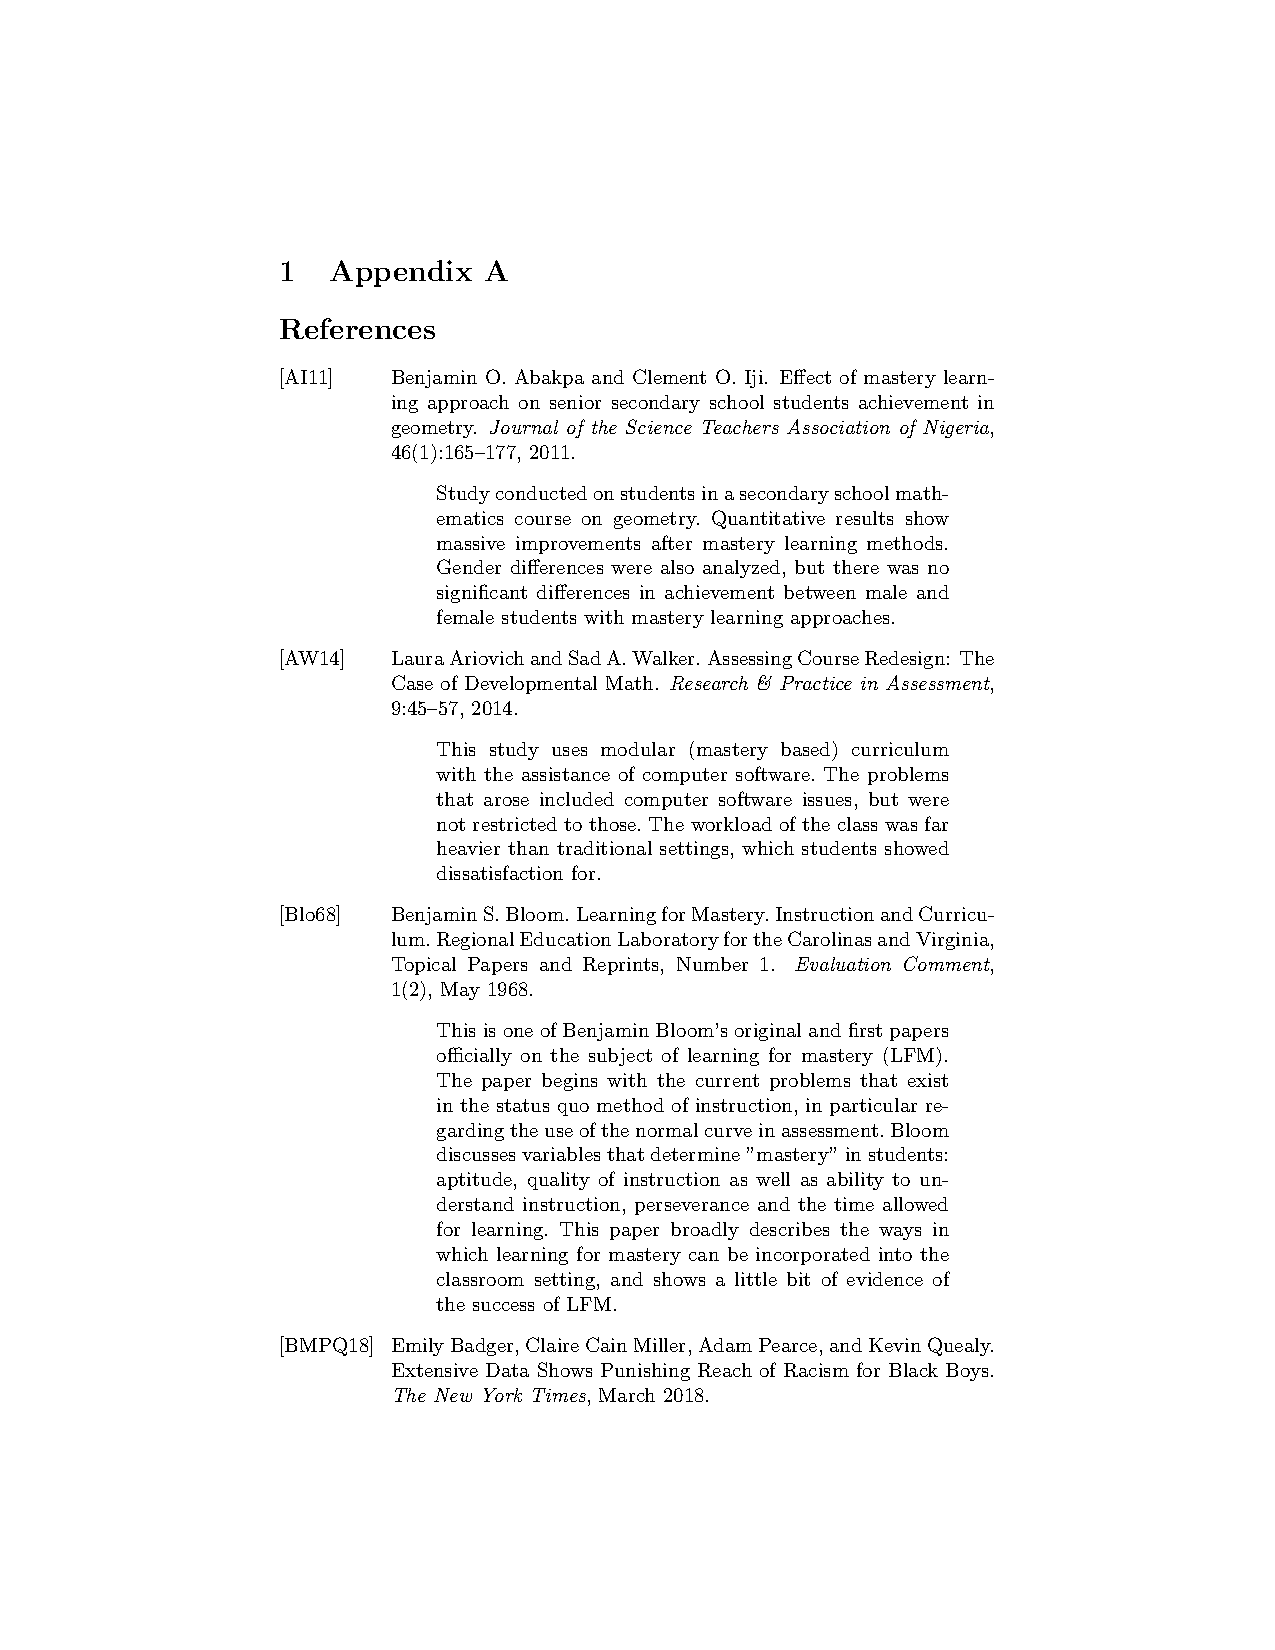
\includepdf[pages=-]{thesis_midterm_jlee.pdf}
\end{document}
